\chapter{Domain-Specific Language} % (fold)
\label{cha:dsl}

In this chapter we present some fundamentals about Domain-Specific Language~(DSL) and
a language used as interface with the users and self-tuning.

A \textit{DSL} is a way to approach some specific
context through appropriate notations and abstractions~\cite{deursen:2000}. DSL
transforms a particular problem domain into a context intelligible for expert
users that can work in a familiar environment.

Problem domain is a crucial term of DSL that requires prior background of the
developers in the specific context. The developers must be expert in the domain
in order to develop a DSL that cover the features required for the users. There are
a lot of examples of DSLs in differents domains: (LEX, YACC, Make, SQL,
HTML, CSS, LATEX, etc.)~\cite{bentley:1986}.

DLSs normally focus on specific domains, containing notations and specific abstractions.
Also it is a \textit{small} and \textit{declarative} language. A
DSL can be extended to different domains. Such DSL is called general-purpose
language (GPL), because its expressiveness power is not restrict to
an exclusive domain, examples of such DSLs are Cobol and Fortran, which
could be viewed as languages focused on the domain of business and scientific
programming  ~\cite{deursen:2000}.

DSL are used in several areas, such as Software Engineering, 
Artificial Intelligence, Computers Architecture~(in this area a
good exemple is VHSIC Hardware Description Language (VHDL), where VHSIC stand for 
{\bf V}ery {\bf H}igh {\bf S}peed {\bf I}ntegrated {\bf C}ircuits), Database
Systems~(SQL, Datalog, QBE, Bloom), Network~(where its
protocols are examples of DSLs), Distribuited Systems, Multi-Media
and among others. A current area that have been emerged recently is \textbf{Big Data}.
This area may be considered as a sub area of Database, but is has many
particularities that involve a mix features of Database and Distributed Systems.

\section{DSL Design Methodology}

The first step to create a new DSL consists in identifing the problem domain. Depending on
the context, it is not trivial to abstract the complete knowledge of the domain, because
the developers must have a deep prior knowledge of the context, so considering all
variables and intrinsics aspects belonging to the domain. Furthermore, sometimes
the context can cover more than one domain (for example the GPLs). In other cases
the correct abstraction of the domain is fast and there is not room for doubts
and equivocation. In both cases the foreknowledge of the developers is the factor
that influences the most the quality of the resulting DSL.

After identifying the problem domain developers must abstract all relevant 
aspects from it. For example {\it VHDL}, group semantic notations and operations
on logical circuit that allows to express logical components: gates circuits, bus, datapath and
control signals. With these four components we can describe any logical circuit
since a ALU~(Arithmetic Logic Unit), register bank till one complex microprocessor. 

The next step consists in designing a DSL that expresses applications in the domain. DSL
will have limited concepts which are all focused on the specific domain. To
design the DLS, it is necessary to analyse the relationship between it and the existing
languages. According to~\cite{mernik:2005}, there are some design patterns to
develop a DSL based on existing languages that is represented by figure ~\ref{fig:patterns}.

\begin{figure}[htbp]
        \centering
        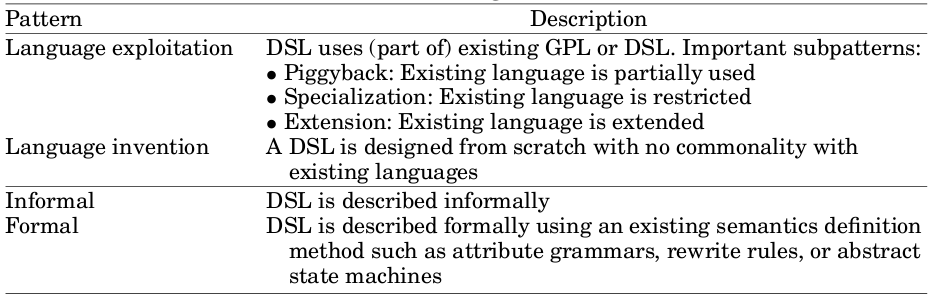
\includegraphics[width=\columnwidth]{img/designPatterns.png}
        \caption{Design patterns - Figure extracted from~\cite{mernik:2005}.}\label{fig:patterns}
\end{figure}

In the implementation, a library with the semantic notations are built
together with a compiler that perfoms the lexical, syntactic and semantic analysis, 
after converting the DSL programs to sequence of library calls. Generally the library
and the compiler are built with support of the tools or framework developed
for this purpose. Xtext~\cite{xtext} and Groovy~\cite{groovyDSL, groovyDSLBook}
are examples of tools to develop DSLs.

\section{Context Transformation}
\label{sec:contextTrans}

Our context is focused on Hadoop environment that have its own particularities. Thus,
a context transformation is mandatory to implement the bacterionlogical algorithm
on such environment.

On Hadoop there is huge set of configuration parameters, we called one specific 
parameter as \textit{knob}. A job use several knobs which we called as set of knobs. 
When sets of knobs are agglomerate we have a population of set of knobs.

In the context tranformation, each component of genetic
context was translated to one component of Hadoop environment. Figure~\ref{fig:transformation}
shows that a gene is transformed into a knob,
an individual (which is a set of genes) is transformed into a set of knobs and,
an individuals population is transformed into a population of set of knobs.

\begin{figure}[htbp]
        \centering
        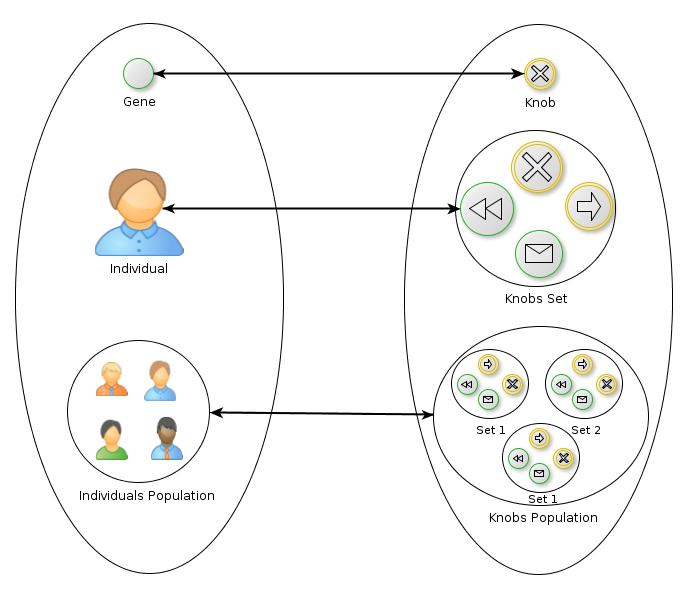
\includegraphics[width=\columnwidth]{img/transformation.jpg}
        \caption{Context transformation.}\label{fig:transformation}
\end{figure}

An interesting characteristic of the tranformation is its bijection that one
component in the genetic domain is translated to one component in Hadoop domain. Beyond
that the transformation has inversion property, i.e, all components in Hadoop domain
can be translated to respective components in genetic domain. That properties
represent compatibility between both domains and somewhat a good representativeness.
\\
\\
\\
\\
\\
\\
\\
%-------------------------------------------------------------------------------
% Put here one formal teorem and a prof for the afirmation above. ^^^^^^^^^^^^^^
%-------------------------------------------------------------------------------
\section{DSL Proposal}

Our DSL proposal is based on the \textbf{Xtext} framework~\cite{xtext}. It requires
to define a grammar and rules for the specific domain. The base of the DLS is the
self-tuning using BA. So our effort aims to describe rules to represent all aspects
and components required for self-tunning.

Our domain has the following components:

\begin{itemize} 
    \item The job with its properties;
    \item The knobs;
    \item The knob with own type, minimum and maximum thresholds and its initial value.
\end{itemize}

Based on these components we present a preliminary version of our DSL:

\singlespacing
\begin{listing}[H]
\begin{minted}[mathescape,frame=lines,framesep=2mm,fontfamily=courier,fontsize=\scriptsize]{python}
DomainModel:
	job=Job;
	
Job:
	'Job' name=ID '{'
        setProperties+=Properties*
		setKnobs+=Knobs*
	'}'
;

Properties:
    'Properties' '{'
        properties+=Property
    '}'

Property:
    name=ID Value
;

Value: String;


Knobs:
	'knobs' '{'
		knobs+=Knob*
	'}' 
;

Knob:
	 name=ID Type
;

Type:
	IntType | FloatType | BoolType
;

IntType:
	'int' MinInt MaxInt '=' INT
;
MaxInt: INT;
MinInt: INT;

FloatType:
	'float' MinFloat MaxFloat '=' Float
;
MaxFloat: Float;
MinFloat: Float;

Float:
	INT*'.'INT*
;

BoolType:
	'boolean' '=' Boolean
;
Boolean:
	'true' | 'false' 
;

\end{minted}
\caption{Initial DSL proposal} 
\label{listing:dlsProposal}
\end{listing}

Oll the rules forming our grammar are presented below:
\begin{enumerate}
	\item
		\singlespacing
		\begin{listing}[H]
		\begin{minted}[mathescape,frame=lines,framesep=2mm,fontfamily=courier,fontsize=\scriptsize]{python}
			DomainModel:
				job=Job;
		\end{minted}
		\label{listing:modelRule}
		\end{listing}

		The first rule in a grammar is always used as the entry or starting rule.
		It espresses that the \textbf{DomainModel} contains one element \textbf{Job}
		assigned to a feature called \textit{job}.

	\item
		\singlespacing
		\begin{listing}[H]
		\begin{minted}[mathescape,frame=lines,framesep=2mm,fontfamily=courier,fontsize=\scriptsize]{python}
			Job:
                'Job' name=ID '{'
                    setProperties+=Properties*
                    setKnobs+=Knobs*
                '}'
            ;	
		\end{minted}
		\label{listing:modelRule}
		\end{listing}

		The rule \textbf{Job} starts with the definition of a keyword ({\it Job})
		followed by a name. Between brackets the job contains one indefinite number
		(*) of \textbf{Properties} and \textbf{Knobs} which will be added (+=) to
        a feature called setProperties and setKnobs, respectively.

    \item
		\singlespacing
		\begin{listing}[H]
		\begin{minted}[mathescape,frame=lines,framesep=2mm,fontfamily=courier,fontsize=\scriptsize]{python}

            Properties:
                'Properties' '{'
                    properties+=Property
                '}'
            ;
		\end{minted}
		\label{listing:modelRule}
		\end{listing}

        The rule {\bf Properties} starts with the definition of a keyword {\bf Properties}
		and between brackets contains one indefinite number (*) of \textbf{Property}
		which will be added~(+=) to a feature called properties.

    \item
		\singlespacing
		\begin{listing}[H]
		\begin{minted}[mathescape,frame=lines,framesep=2mm,fontfamily=courier,fontsize=\scriptsize]{python}

            Property:
                name=ID Value
            ;

            Value: String;
		\end{minted}
		\label{listing:modelRule}
		\end{listing}

        These two rules are used to describe job properties, each property has an
        ID followed by its value. The value is an String.

	\item
		\singlespacing
		\begin{listing}[H]
		\begin{minted}[mathescape,frame=lines,framesep=2mm,fontfamily=courier,fontsize=\scriptsize]{python}
			Knobs:
				'knobs' '{'
					knobs+=Knob*
				'}' 
			;
		\end{minted}
		\label{listing:modelRule}
		\end{listing}

		The rule \textbf{Knobs} starts with the definition of a keyword {\bf knobs}
		and between brackets contains one indefinite number (*) of \textbf{Knob}
		which will be added (+=) to a feature called knobs.

	\item
		\singlespacing
		\begin{listing}[H]
		\begin{minted}[mathescape,frame=lines,framesep=2mm,fontfamily=courier,fontsize=\scriptsize]{python}
			Knob:
				 name=ID Type
			;
		\end{minted}
		\label{listing:modelRule}
		\end{listing}

		The rule \textbf{Knob} contain one name followed by a \textbf{Type} with
		your peculiarities explained below.

	\item
		\singlespacing
		\begin{listing}[H]
		\begin{minted}[mathescape,frame=lines,framesep=2mm,fontfamily=courier,fontsize=\scriptsize]{python}
			Type:
				IntType | FloatType | BoolType
			;
		\end{minted}
		\label{listing:modelRule}
		\end{listing}

		The rule \textbf{Type} can accept three type: \texttt{integer}, \texttt{float} or \texttt{boolean},
		this three are all possibles types on hadoop parameters configuration.

	\item
		\singlespacing
		\begin{listing}[H]
		\begin{minted}[mathescape,frame=lines,framesep=2mm,fontfamily=courier,fontsize=\scriptsize]{python}
			IntType:
				'int' MinInt MaxInt '=' INT
			;
			MaxInt: INT;
			MinInt: INT;
		\end{minted}
		\label{listing:modelRule}
		\end{listing}

		These three rules are used for integer types, the rule \textbf{IntType}
		starts with the keyword {\bf int} followed by your respective minimum
		and maximum possibles values. In sequence there is the keyword {\bf '='}
		and the initial value for the knob.

	\item
		\singlespacing
		\begin{listing}[H]
		\begin{minted}[mathescape,frame=lines,framesep=2mm,fontfamily=courier,fontsize=\scriptsize]{python}
			FloatType:
				'float' MinFloat MaxFloat '=' Float
			;
			MaxFloat: Float;
			MinFloat: Float;

			Float:
				INT*'.'INT*
			;
		\end{minted}
		\label{listing:modelRule}
		\end{listing}

		These four rules are used for float types, the rule \textbf{FloatType} is
		similar the IntType rule, it starts with the keyword {\bf float} followed
		by your respective minimum and maximum possibles values. In sequence there
		is the keyword {\bf '='} and the initial float value for the knob. The rule
		{\bf FloatType} expresses the float format.

	\item
		\singlespacing
		\begin{listing}[H]
		\begin{minted}[mathescape,frame=lines,framesep=2mm,fontfamily=courier,fontsize=\scriptsize]{python}
			BoolType:
				'boolean' '=' Boolean
			;
			Boolean:
				'true' | 'false' 
			;
		\end{minted}
		\label{listing:modelRule}
		\end{listing}

		The last rule {\bf BoolType} expresses the boolean type, it starts with
		the keyword {\bf boolean} followed by signal of \textbf{'='} and the initial
		boolean	value that can be {\bf true} or {\bf false}.

\end{enumerate}
